Based on the 3 rules we further implement other optimizations of our own, and extend the model to include more complicated rules as proposed in section~\ref{sec:proposal}. 
\subsection{Performance}
Iterating all flock mates for each boid per frame is too expensive and may cause a lot of lag or system crashes. We took Sebastian Lague’s project as a reference and implemented a GPU based multi-thread iteration for calculating the three key parameters mentioned above. Each boid is assigned a single thread on the GPU and all boids run parallel on GPU and iterates simultaneously with global synchronization at the very end. Since each boid is independent of other boids, and do not update other boids in any way, the problem becomes embarrassingly parallel and very efficient on the GPU.

\subsection{Realistic}
We also add a random force to each boid every 20 frames. In some situation(e.g. When the flock move straight forward for a time), the boids make no change and cause the whole flock look too ordered and becomes even sterile. So an uneven force with random direction is added to add realism to the flock motion. This force is not designed to completely break the flock order and reform again but to downgrade the precision of computer calculated simulation and make the motion more realistic. We also tried to implement a gravity to the system, but we found that this had almost no effect to the system in play.

\subsection{Avoid Obstacle}

The interaction with the obstacle object is the most interesting part of the whole simulation. It makes the flock motion more random and unpredictable when it comes across an object with complex shape. Sometimes the boids further divide into several smaller groups but the whole motion looks still realistic and in later timesteps you can observe them forming back into one single flock. 
\begin{center}
  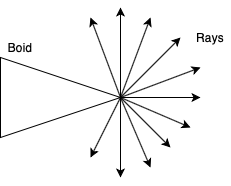
\includegraphics[width=5cm, height=3cm]{{docs/fig/rays.png}}
  \end{center}
The strategy to achieve this is complicated. Craig W. Reynolds mentioned two different attempts: force field model and steer-to-avoid, and we implemented the latter one since it has a better performance. We designed several rays sending outwards from the boids to detect if there are obstacles ahead. The challenge is detecting the collision of rays on the surface of an object could be very expensive if the object is polyhedral. It turns to be even more complicated to further figure out the direction for a boid to avoid the object, especially in a 3D environment. We simplify this question by casting the obstacle into a sphere. In this case for each ray sending from the boid, the obstacle could be measured as a circle on a 2D panel with this ray. With this casting process, we solve 2 problems together: the complexity of directions in 3D and arbitrary shape of obstacles. 
\begin{center}
  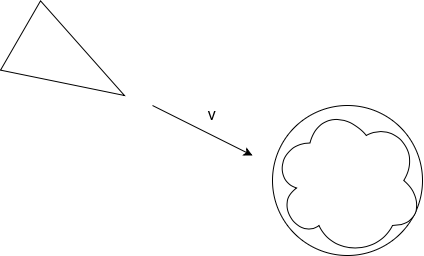
\includegraphics[width=5cm, height=3cm]{{docs/fig/avoid1.png}}
\end{center}
When an obstacle is detected, a normalized force will be added to the boid on the same panel of the detection ray. This force is designed to turn the heading of the current boid and the angle it turns will be based on the golden ratio. In some simplified cases, for example, if a boid heading perpendicular to a flat surface, the boid will steer a golden spiral to avoid a collision. This is designed to avoid sharp turns and make the whole process smooth and natural. Since the flock is still maintaining during the avoid process, the avoid force is added based on the 3 rules and it is not necessary to worry about whether the force from the 3 rules may affect the performance of avoiding.
\begin{center}
  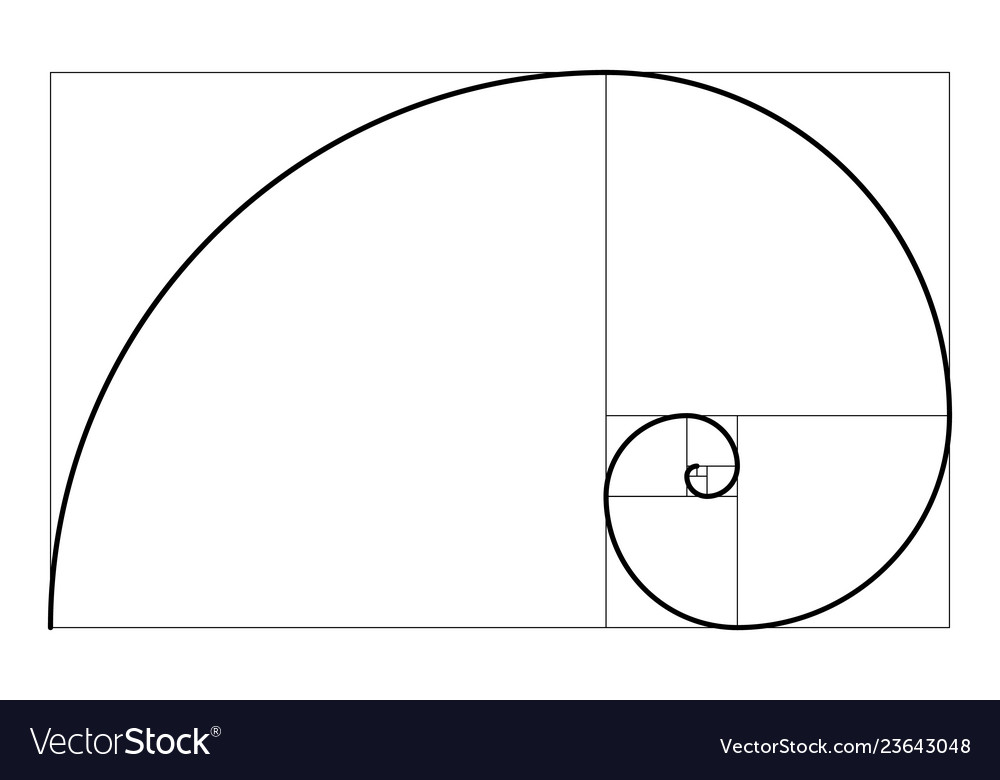
\includegraphics[width=4cm, height=3cm]{{docs/fig/golden spirial.jpg}}
\end{center}

\subsection{Prey and Predator}

To test the durability of our system, we introduced a prey and predator into our system to simulate a real natural scene.

The prey randomly picks a point in the 3D scene and move toward that point. To make the motion of prey smooth and real, we implement a force from the position of prey to the target point on prey each frame. When the prey reaches the target, another point will be randomly picked. The flock chases the prey in a similar way. A force heading the prey is added on every boid each frame together with 3 rules. To make the scene more simple we set the speed of prey always greater than the boids so the flock never catches up. 

We also added a predator to chase the flock. The predator is always heading the center of the flock and the strategy is exactly the same as boid chasing prey. Each boid gets an updated predator position each frame. If the distance of predator is less than an avoid radius an escape force will be added toward an opposite direction of the predator on boid. The difference between avoiding predators and obstacles is the boids do not follow three rules when escaping predators. We notice that three rules should not be implemented to simulate avoid predators since alignment and cohesion always playing a dominant role in boid motion. Even we set an escape weight and set it 10 times more than the weights for three rules, the flock still does not show a distinct escaping motion while predator approaches. In our implementation, we only reserve the separation part and set a significantly higher speed to boid, in order to match a similar escaping scene from the natural world.

\subsection{Local Animations}

To add to the realism, we are able to import any custom blender model into our 3D scene. So the same simulation can be used for birds or fish or any sort of flock motion, and also incorporate hand-crafted local animations for each model while animating the larger flock. Since our system uses a GPU to process some of the more compute intensive tasks, it is easily able to handle the minute local animations that further add realism.

There's also further research needed to automate such realism for a flock simulation, similar to what have been done for human crowd simulation with the little random arm and shoulder gestures.